\documentclass[11pt,a4paper,twoside]{article} %twocolumn
\usepackage[francais]{babel}
\usepackage[babel=true,kerning=true]{microtype}
\usepackage[utf8]{inputenc}
\usepackage[T1]{fontenc}
\usepackage{lmodern}
\usepackage[top=2cm,bottom=2.2cm,right=2.2cm,left=2.2cm]{geometry}
\usepackage{graphicx}
\usepackage{fig-planes}
\usepackage{tikzfmv}
\graphicspath{{./img/}}
%%%%%%%%%%%%%%%%%%%%%%%%%%%%%%%%%%%%%%%%%%%%%%%%%%%%%%%%%%%%%%%%%%%%%%%%%%%%%%%%
%%%%%%%%%%%%%%%%%%%%%%%%%%%%%%%%%%%%%%%%%%%%%%%%%%%%%%%%%%%%%%%%%%%%%%%%%%%%%%%%
\usepackage{examen}
%Modifier les variables suivantes :
\annee{2024-2025}                  
\promo{IngéSUP}                                        % ex. IngéSUP, IngéSPE, Ingé1
\module{\fr{Systèmes Techniques}{Technical Systems}}
\epreuve{Midterm}                                      % ex. MidTerm, FinalExam, Rattrapage
\titreEval{\fr{Systèmes Mécaniques - Cinématique}
              {Mechanical Systems - Kinematics}}       % ex. Dynamique et Déformation
\dureeEval{2}                                          % ex. 2 (en nombre d'heures)
\documentautorise{false}                               % les documents sont-ils autorisés true or false 
\moyencalcul{false}                                    % les moyens de calculs sont-ils autorisés
\dispositions{true}                                    % Remarque en cas de découverte de coquille
\esme{true}                                            % examen ESME true or false
\grille{true}                                          % document réponse true or false
\corrige{false}
%%%%%%%%%%%%%%%%%%%%%%%%%%%%%%%%%%%%%%%%%%%%%%%%%%%%%%%%%%%%%%%%%%%%%%%%%%%%%%%%
\pagestyle{esmestyle}
\begin{document}
\maketitle
\thispagestyle{esmestyle}
%%%%%%%%%%%%%%%%%%%%%%%%%%%%%%%%%%%%%%%%%%%%%%%%%%%%%%%%%%%%%%%%%%%%%%%%%%%%%%%%
%%%%%%%%%%%%%%%%%%%%%%%%%%%%%%%%%%%%%%%%%%%%%%%%%%%%%%%%%%%%%%%%%%%%%%%%%%%%%%%%
\exercice{\fr{Dérivation Vectorielle}{Vector derivation} \textbf{(5 pts)}}
%%%%%%%%%%%%%%%%%%%%%%%%%%%%%%%%%%%%%%%%%%%%%%%%%%%%%%%%%%%%%%%%%%%%%%%%%%%%%%%%
\fr{On considère trois repères de bases ($R_0,R_1,R_2$) déduits les uns des autres par rotation 
comme le précisent les deux figures planes de calcul suivantes :}
{Three reference frames ($R_0,R_1,R_2$) are considered, derived from one another by rotation, as specified in the 
following two basis change representation:}
\begin{center}
\begin{tikzpicture}
    \figplanes[][theta][][1][col1][0][col5]{[x][y][z][A]}
\end{tikzpicture}
\begin{tikzpicture}
    \figplanes[][phi][][2][col4][1][col1]{[z][x][y][A]}
\end{tikzpicture}
\end{center}
\fr{On se donne le vecteur $\ap$ tel que :}
   {Let the vector $\ap$ be:}
\[
\ap=\rho(t)\xx{2}
\]
\fr{L'objectif de cet exercice est d'appliquer les régles de calculs de la 
    dérivation vectorielle pour déterminer la variation de ce vecteur dans la base 0.\\}
   {The objective of this exercise is to apply the rules of vector calculus 
    to determine the variation of this vector relatively to $R_0$.\\}
%%%%%%%%%%%%%%%%%%%%%%%%%%%%%%%%%%%%%%%%%%%%%%%%%%%%%%%%%%%%%%%%%%%%%%%%%%%%%%%%
\question{\fr{Donner le vecteur vitesse de rotation $\Om{1/0}$ et $\Om{2/1}$}
             {Give the instantaneous rotation vector $\Ome{0}{1}$ and $\Ome{1}{2}$ 
             (or in french: $\Om{1/0}$ et $\Om{2/1}$).} [1 pt]}
%%%%%%%%%%%%%%%%%%%%%%%%%%%%%%%%%%%%%%%%%%%%%%%%%%%%%%%%%%%%%%%%%%%%%%%%%%%%%%%%
\grillereponse[3cm]{$\Om{1/0}=\dtheta\zz{0}$\\$\Om{2/1}=\dphi\yy{1}$}
%%%%%%%%%%%%%%%%%%%%%%%%%%%%%%%%%%%%%%%%%%%%%%%%%%%%%%%%%%%%%%%%%%%%%%%%%%%%%%%%
\question{\fr{Déterminer le vecteur vitesse de rotation   $\Om{2/0}$}
             {Determine the instantaneous rotation vector $\Ome{0}{2}$ (or in french: $\Om{2/0}$)} [1 pt]}
         
\grillereponse[1cm]{$\Om{2/0}=\Om{2/1}+\Om{1/0}=\dtheta\zz{0}+\dphi\yy{1}$}
%%%%%%%%%%%%%%%%%%%%%%%%%%%%%%%%%%%%%%%%%%%%%%%%%%%%%%%%%%%%%%%%%%%%%%%%%%%%%%%%
\question{\fr{Donner la dérivée du vecteur unitaire $\xx{2}$ par rapport aux vecteurs de base $\bas{0}$}
             {Give the derivative of the unit vector $\xx{2}$ expressed in basis $\bas{0}$}. [1.5 pts]}
%%%%%%%%%%%%%%%%%%%%%%%%%%%%%%%%%%%%%%%%%%%%%%%%%%%%%%%%%%%%%%%%%%%%%%%%%%%%%%%%
\grillereponse[3.5cm]{
\[
    \deviV{\xx{2}}{}{R_0}=\Om{2/0}\land\xx{2}=\dtheta\zz{0}+\dphi\yy{2}\land\xx{2}
\]
\[
    \boxed{\deviV{\xx{2}}{}{R_0}=-\dphi\zz{2}+\dtheta\cos\phi\yy{1}}
\]}
%%%%%%%%%%%%%%%%%%%%%%%%%%%%%%%%%%%%%%%%%%%%%%%%%%%%%%%%%%%%%%%%%%%%%%%%%%%%%%%%
\question{\fr{À partir des résultats précédents, déterminer la dérivée du vecteur $\deviV{\ap}{}{R_0}$.}
             {From the previous results, determine the derivative of the vector $\dif{R_0}{\ap}$ (or in french : $\deviV{\ap}{}{R_0}$).} [1.5 pts]}
%%%%%%%%%%%%%%%%%%%%%%%%%%%%%%%%%%%%%%%%%%%%%%%%%%%%%%%%%%%%%%%%%%%%%%%%%%%%%%%%
\grillereponse[3.5cm][\clearpage][][\clearpage]{
\[
    \deviV{\ap}{}{R_0}=\drho\xx{2}+\rho\deviV{\xx{2}}{}{}
\]
\[
    \boxed{\deviV{\ap}{}{R_0}=\drho\xx{2}+\rho\dtheta\cos\phi\yy{2}-\rho\dphi\zz{2}}
\]}
%%%%%%%%%%%%%%%%%%%%%%%%%%%%%%%%%%%%%%%%%%%%%%%%%%%%%%%%%%%%%%%%%%%%%%%%%%%%%%%%
\exercice{\fr{Cinématique d'un moulin à farine}
             {Kinematic of a flour mill} \textbf{(10 pts)}}
%%%%%%%%%%%%%%%%%%%%%%%%%%%%%%%%%%%%%%%%%%%%%%%%%%%%%%%%%%%%%%%%%%%%%%%%%%%%%%%%
\fr{%
Le dispositif utilisé pour écraser les graines de céréales comporte trois
solides principaux, présentés sur l'ébauche de schéma ci-dessous :
}{The device used to crush cereal grains has three main solids,
shown in the draft diagram below:}
\begin{itemize}
    \setlength\itemsep{0.1em}
    \item \fr{Au bâti \textbf{1} est associé le repère $\rep{O}{1}$.}
          {Solid \textbf{1} is associated the frame $\rep{O}{1}$.}
    \item \fr{L'arbre \textbf{2} est lié au bâti 1 par une liaison pivot glissant
          d'axe $\axe{O}{z}[1]$. On lui associe le repère $\rep{B}{2}$,
          tel que $\zz{2}=\zz{1}$; on pose $\alpha= (\xx{1},\xx{2})$ et $\ob=\mu \zz{1}$.
          La distance OB n'est pas fixe pour permettre au mécanisme de fonctionner.}
          {The shaft \textbf{2} is linked to structure \textbf{1} by a sliding pivot joint
          of axis $\axe{O}{z}[1]$. The frame $\rep{B}{2}$ is associated with it,
          such that $\zz{2}=\zz{1}$; we set $\alpha= (\xx{1},\xx{2})$ and $\ob=\mu \zz{1}$.
          The distance OB is not fixed to allow the mechanism to operate}
   \item \fr{La meule \textbf{3}, de rayon $R$, est liée à l'arbre \textbf{2} par une liaison
          pivot d'axe $\axe{B}{x}[2]$. On lui associe le repère
          $\rep{B}{3}$, tel que $\xx{3}=\xx{2}$ et on pose $\beta= (\yy{2},\yy{3})$.}
          {The wheel \textbf{3}, of radius $R$, is connected to the shaft \textbf{2} by a pivot
          joint of axis $\axe{B}{x}[2]$. The frame $\rep{B}{3}$ is associated with it,
          such that $\xx{3}=\xx{2}$ and we set $\beta= (\yy{2},\yy{3})$.}
   \item \fr{Finalement, la meule \textbf{3} est en contact avec le bâti par une liaison 
          linéaire rectiligne (ou dites encore cylindre/plan) d'axe $\axe{B}{x}[3]$}
          {Finally, the grinding wheel \textbf{3} is in contact with the frame by a 
          cylindrical slider (or also called cylinder/plane contact) with axis $\axe{B}{x}[3]$}
\end{itemize}
\fr{Soit I l'un des points de contact appartenant au segment de la tranche de la meule, on pose $\oi=\lambda\xx{2}$.}
   {Let I be one of the contact points belonging to the segment of the wheel slice, we set $\oi=\lambda\xx{2}$.}
\begin{figure}[h]
    \centering
    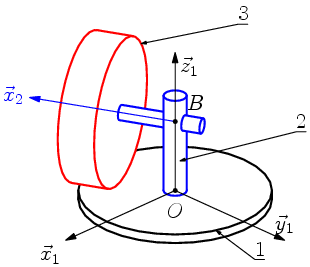
\includegraphics[width=0.39\linewidth]{fig/ebauche-schema_moulin.png}
    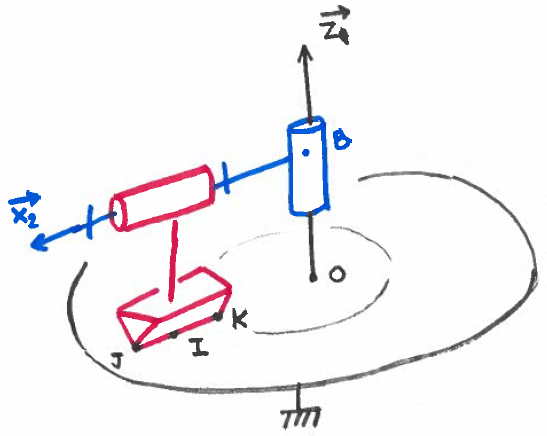
\includegraphics[width=0.39\linewidth]{fig/schema_meule.png}
    \caption{\fr{(à gauche) Ebauche d'un moulin à farine (à droite) et son schéma cinématique.}
                {(left) Sketch of a flour mill and (right) his kinematic diagram}}
\end{figure}
%%%%%%%%%%%%%%%%%%%%%%%%%%%%%%%%%%%%%%%%%%%%%%%%%%%%%%%%%%%%%%%%%%%%%%%%%%%%%%%%
\question{\fr{Tracer le graphe de liaison de ce mécanisme}
             {Draw the link diagram of this mechanism} [1pt]}
%%%%%%%%%%%%%%%%%%%%%%%%%%%%%%%%%%%%%%%%%%%%%%%%%%%%%%%%%%%%%%%%%%%%%%%%%%%%%%%%
\grillereponse[9cm][][\clearpage]{
\begin{center}
    \begin{tikzpicture}[scale=2.0]
        \scSolideExt[bati]{black,ultra thick}
        \scSolides{bati}{bati}\scBati[-90]{A}{-1,0}
        \node[state,black,line width=1.5pt] (S0) {$1$};
        \node[state,blue,line width=1.5pt,right=3.5cm of S0,yshift=-2cm] (S1) {$2$};
        \node[state,red,line width=1.5pt,right=3.5cm of S1,yshift=2cm] (S2) {$3$};
        \draw[every loop,-,line width=1.5pt]  (S0) edge [bend right] node[text width=4cm,below left,align=center]
        {\small Pivot glissant d'axe $\axe{O}{z}[1]$ } (S1);
        \draw[every loop,-,line width=1.5pt]  (S1) edge [bend right] node[midway,below right,text width=4cm,align=center]
        {\small Pivot d'axe $\axe{B}{x}[2]$} (S2);
        \draw[every loop,-,line width=1.5pt]  (S0) edge [bend left] node[midway,above,text width=5cm,align=center]
        {\small Liaison linéaire rectiligne d'axe $\axe{B}{x}[3]$} (S2);
        \draw[bati] (A) -- (S0);
        \draw[bati] (A) -- (S0);
    \end{tikzpicture} 
\end{center}}
%%%%%%%%%%%%%%%%%%%%%%%%%%%%%%%%%%%%%%%%%%%%%%%%%%%%%%%%%%%%%%%%%%%%%%%%%%%%%%%%
\question{\fr{Tracer les figures planes permettant de représenter les paramètres d'orientation.}
             {Draw the basis change representations associated to the motions.} 
[2 pts]}
%%%%%%%%%%%%%%%%%%%%%%%%%%%%%%%%%%%%%%%%%%%%%%%%%%%%%%%%%%%%%%%%%%%%%%%%%%%%%%%%
\grillereponse[6cm]{
\begin{center}
\begin{tikzpicture}
    \figplanes[b][alpha][][2][col1][1][col5]{[x][y][z][O][]}
\end{tikzpicture}
\hspace{1cm}
\begin{tikzpicture}
    \figplanes[b][beta][][3][col4][2][col1]{[y][z][x][B][]}
\end{tikzpicture}
\end{center}}
%%%%%%%%%%%%%%%%%%%%%%%%%%%%%%%%%%%%%%%%%%%%%%%%%%%%%%%%%%%%%%%%%%%%%%%%%%%%%%%%
\question{\fr{Donner les torseurs cinématiques associés aux 
              mouvements des solides 2/1 et 3/2 au point B (c'est à dire ceux associés aux pivots).
              \emph{Attention la distance OB n'est pas fixe:  $\ob=\mu(t) \zz{1}$ }}
             {Give the kinematic torsors associated to the movements 
              of 3 relatively to 2 and 2 relatively to 1 at point O (i.e. those associated with the hinges).
              \emph{Warning OB length is not constant: $\ob=\mu(t) \zz{1}$ }} [2 pts]}
%%%%%%%%%%%%%%%%%%%%%%%%%%%%%%%%%%%%%%%%%%%%%%%%%%%%%%%%%%%%%%%%%%%%%%%%%%%%%%%%
\grillereponse[6cm]{%
\[
\torC{2/1}{B}=\begin{Bmatrix}\Om{2/1}\\[0.5em]\TCV{B}{2}{1}\end{Bmatrix}_\mathrm{B}
             =\begin{Bmatrix}\dalpha\zz{1}\\[0.5em]\dmu\zz{1}\end{Bmatrix}_\mathrm{B}
\]
\[
\torC{3/2}{B}=\begin{Bmatrix}\Om{3/2}\\[0.5em]\TCV{B}{3}{2}\end{Bmatrix}_\mathrm{B} 
             =\begin{Bmatrix}\dbeta\xx{2}\\[0.5em]\vnull\end{Bmatrix}_\mathrm{B}
\]}
%%%%%%%%%%%%%%%%%%%%%%%%%%%%%%%%%%%%%%%%%%%%%%%%%%%%%%%%%%%%%%%%%%%%%%%%%%%%%%%%
\question{\fr{Déterminer les vitesses $\TCV{I}{2}{1}$ et $\TCV{I}{3}{2}$}
             {Determine the velocities $\TVe{1}{2}{I}$ and $\TVe{2}{3}{I}$ (in french: $\TCV{I}{2}{1}$ and $\TCV{I}{3}{2}$)}. [2 pts]}
%%%%%%%%%%%%%%%%%%%%%%%%%%%%%%%%%%%%%%%%%%%%%%%%%%%%%%%%%%%%%%%%%%%%%%%%%%%%%%%%
\grillereponse[6cm][\clearpage][\clearpage]{
\[
    \TCV{I}{2}{1}=\TCV{B}{2}{1} + \Om{2/1}\land\bi = \dmu\zz{1} + \lambda\dalpha\yy{2}  
\]
\[
    \TCV{I}{3}{2}= \Om{3/2}\land\bi = \mu\dbeta\yy{2}
\]
}
%%%%%%%%%%%%%%%%%%%%%%%%%%%%%%%%%%%%%%%%%%%%%%%%%%%%%%%%%%%%%%%%%%%%%%%%%%%%%%%%
\question{\fr{Déterminer la vitesse $\TCV{I}{3}{1}$ par composition du mouvement}
             {Determine the velocity $\TVe{1}{3}{I}$ (in french: $\TCV{I}{3}{1}$) by using the composition of velocities}. [1 pt]}
%%%%%%%%%%%%%%%%%%%%%%%%%%%%%%%%%%%%%%%%%%%%%%%%%%%%%%%%%%%%%%%%%%%%%%%%%%%%%%%%
\grillereponse[4cm]{
\[
    \TCV{I}{3}{1}=\TCV{I}{3}{2} + \TCV{I}{2}{1}
\]
\[
    \TCV{I}{3}{1}=(\lambda\dalpha+\mu\dbeta)\yy{2}+\dmu\zz{1}
\]}
%%%%%%%%%%%%%%%%%%%%%%%%%%%%%%%%%%%%%%%%%%%%%%%%%%%%%%%%%%%%%%%%%%%%%%%%%%%%%%%%
\question{\fr{Dans quel cas cette vitesse est orthogonal à $\zz{1}$ ? Autrement dit, 
              déterminer la condition pour que $\TCV{I}{3}{1}\cdot\zz{1}=0$}
             {In which case is this velocity 
              orthogonal to $\zz{1}$? In other words, determine the condition
              to have $\TVe{1}{3}{I}\cdot\zz{1}=0$ (in french: $\TCV{I}{3}{1}\cdot\zz{1}=0$)}. [1 pt]}
%%%%%%%%%%%%%%%%%%%%%%%%%%%%%%%%%%%%%%%%%%%%%%%%%%%%%%%%%%%%%%%%%%%%%%%%%%%%%%%%
\grillereponse[3cm]{
\[
    \TCV{I}{3}{1}\cdot\zz{1} = 0 \Leftrightarrow \dmu = 0 
\]
La distance entre OB doit être une constante.}
%%%%%%%%%%%%%%%%%%%%%%%%%%%%%%%%%%%%%%%%%%%%%%%%%%%%%%%%%%%%%%%%%%%%%%%%%%%%%%%%
\question{\fr{Que devient la vitesse $\TCV{I}{3}{1}$ pour $\dmu=0$ ? 
              Et dans ce cas, déterminer une relation pour que $\TCV{I}{3}{1}=\vnull$}
             {What happens to the speed $\TCV{I}{3}{1}$ for $\dmu=0$? And in this case, 
              determine a relationship so that $\TCV{I}{3}{1}=\vnull$} [1 pt]}
%%%%%%%%%%%%%%%%%%%%%%%%%%%%%%%%%%%%%%%%%%%%%%%%%%%%%%%%%%%%%%%%%%%%%%%%%%%%%%%%
\grillereponse[4cm][\clearpage][\clearpage]{
Si $\dmu=0$ alors :
\[
    \TCV{I}{3}{1}=(\lambda\dalpha+\mu\dbeta)\yy{2}
\]
et donc on a $\TCV{I}{3}{1}=\vnull$ si :
\[
    (\lambda\dalpha+\mu\dbeta) = 0
\]}
\end{document}
